\documentclass[conference]{IEEEtran}
\IEEEoverridecommandlockouts
% The preceding line is only needed to identify funding in the first footnote. If that is unneeded, please comment it out.
\usepackage{cite}
\usepackage{amsmath,amssymb,amsfonts}
\usepackage{algorithmic}
\usepackage{graphicx}
\usepackage{textcomp}
\usepackage[T1]{fontenc}
\usepackage{xcolor}
\usepackage{booktabs}
\usepackage{multirow}
\usepackage{tabularx}
\usepackage{stfloats}
\usepackage{hyperref}
\usepackage{tikz}
\usepackage{pgfplots}

\usetikzlibrary{positioning,arrows.meta,shapes.geometric,fit,backgrounds,shapes.misc,calc,decorations.pathreplacing}

\definecolor{managerbg}{RGB}{245,248,252}
\definecolor{managerborder}{RGB}{70,90,120}
\definecolor{semanticcol}{RGB}{255,220,180}
\definecolor{semanticborder}{RGB}{200,120,40}
\definecolor{episodiccol}{RGB}{200,230,255}
\definecolor{episodicborder}{RGB}{40,110,180}
\definecolor{declarativecol}{RGB}{210,240,210}
\definecolor{declarativeborder}{RGB}{40,130,60}
\definecolor{ercol}{RGB}{255,210,210}
\definecolor{erborder}{RGB}{180,50,50}
\definecolor{inputcol}{RGB}{250,240,200}
\definecolor{inputborder}{RGB}{160,130,40}
\definecolor{actioncol}{RGB}{230,210,255}
\definecolor{actionborder}{RGB}{110,60,170}

\pgfplotsset{compat=1.18}

\emergencystretch=10em
\hbadness=10000
\vbadness=10000

\def\BibTeX{{\rm B\kern-.05em{\sc i\kern-.025em b}\kern-.08em
    T\kern-.1667em\lower.7ex\hbox{E}\kern-.125emX}}

\begin{document}
\sloppy

\title{Tri-Mem: Entropy-Routed Modality Matching for Long-Horizon Agent Memory\\
}

\author{\IEEEauthorblockN{Aniruddha Pandey}
    \IEEEauthorblockA{\textit{Department of Computer Science} \\
        \textit{Stevens Institute of Technology}\\
        apandey10@stevens.edu}
    \and
    \IEEEauthorblockN{Xuan Li}
    \IEEEauthorblockA{\textit{Department of Computer Science} \\
        \textit{Stevens Institute of Technology}\\
        xli220@stevens.edu}
    \and
    \IEEEauthorblockN{Amy Thomas}
    \IEEEauthorblockA{\textit{Department of Computer Science} \\
        \textit{Stevens Institute of Technology}\\
        athomas14@stevens.edu}
}

\maketitle

\begin{abstract}
    Current agentic AI systems suffer from context rot and severe token inefficiencies over long-horizon tasks because they force all cognitive functions---rules, episodic interaction history, and exact variables---into a single text-based context window. We introduce Tri-Mem, a research architecture that argues agent memory should not be one-size-fits-all. Tri-Mem assigns distinct cognitive functions to the data modality that appears cheapest and most accurate for that function. Drawing inspiration from human cognitive architecture, Tri-Mem is divided into Semantic Memory (powered by \emph{Memory Sparse Attention} over latent KV chunks) for static rule-following, Episodic Working Memory (utilizing visual bus compression) for chronological interaction history, and Declarative Memory (employing text-based RAG) for exact fact retrieval. Furthermore, we introduce an uncertainty-guided Entropy Router that dynamically routes memory access based on the model's epistemic uncertainty. In our reported NovaCorp AuditBench configuration, Tri-Mem reduces cumulative token cost by 84\% versus the text-only baseline and eliminates the benchmark's measured spatial hallucination and syntactic failure events. To validate the architecture against a public benchmark we additionally evaluate Tri-Mem on the LongMemEval~\cite{longmemeval2024} oracle split (500 questions, six conversational-memory categories), where the modality-routed agent reaches 81.4\% overall and 83.2\% on factual question types under a per-category dispatch-aware LLM judge that pairs a strict paraphrase-tolerant judge for factual categories with a rubric judge for preference questions. On the distractor-loaded \texttt{s\_cleaned} split (${\sim}50$ haystack sessions per task) the same agent projects to the mid-75\% range, with the observed per-category retrieval cost concentrated in multi-session synthesis and temporal reasoning rather than in single-session recall. This modality-to-function mapping offers a structured, ontology-aligned approach to agent memory that decouples cognitive function from a single homogeneous context window.
\end{abstract}

\begin{IEEEkeywords}
    LLM Memory, Conversational Memory, Visual Compression, Retrieval-Augmented Generation, Memory Sparse Attention, Entropy Routing
\end{IEEEkeywords}

\section{Introduction}

As Large Language Models (LLMs) are deployed in increasingly complex, long-horizon agentic systems, they are hindered by a fundamental architectural bottleneck: the homogeneous, text-only context window (Fig.~\ref{fig:motivation}). In standard agentic deployments, developers append standard operating procedures (SOPs), system documentation, multi-turn interaction logs, and retrieved database strings into a single, expanding text prompt. This paradigm induces three cascading failures. First, \textit{context rot} (the "lost in the middle" phenomenon) occurs as conversation history grows, causing models to drop critical instructions \cite{liu2023lost}. Second, systems incur a massive \textit{compute tax} by forcing the model to re-attend to static rulebooks at every turn --- a cost that prefix-cache and paged-KV systems explicitly target~\cite{vllm2023}. Finally, agents experience a \textit{modality-memory mismatch}, where highly verbose textual representations are inefficient for spatial or episodic recall~\cite{deepseekocr,vist2025}, while visually compressed memories suffer lossy recall of exact alphanumeric strings.

To address these challenges, we present \textbf{Tri-Mem}, a modality-matched memory hierarchy for long-horizon agents. The core proposition of Tri-Mem is \textit{Modality-to-Function Mapping}: specific types of agentic thought require specific data modalities to optimize compute and fidelity limits.

We map the architecture directly to human cognitive structures, partitioning memory into three modality-distinct layers:
\begin{enumerate}
    \item \textbf{Semantic Memory (MSA):} A sparse-attention KV chunk layer for static rules and deep reasoning.
    \item \textbf{Episodic Working Memory (Visual Bus):} Compressed image patches for interaction history and spatial navigation.
    \item \textbf{Declarative Memory (RAG):} Discrete text tokens retrieved from a vector database for exact string lookups (e.g., API keys, object IDs).
\end{enumerate}

Furthermore, we introduce an \textit{Entropy Router} that utilizes the model's raw logit confidence (Shannon Entropy) to dynamically route queries to the correct memory layer, preventing costly and latency-heavy LLM-based reasoning for simple memory retrieval.

In our reported NovaCorp AuditBench experiments, replacing the homogeneous text context with a Tri-Mem architecture is associated with longer usable task horizons, lower cumulative token costs, and fewer syntax-related failures than the text-only baseline. We further validate the architecture on \textit{LongMemEval}~\cite{longmemeval2024}, a public benchmark of conversational long-term memory, where Tri-Mem's three-layer routing reaches 83.2\% accuracy on the 470 factual oracle-split questions across five cognitive subtasks (single-session-user, single-session-assistant, multi-session, knowledge-update, and temporal-reasoning), and 81.4\% across all six categories under per-category judge dispatch.

\textbf{Contributions.}
\begin{enumerate}
    \item A modality-routed three-layer memory architecture (MSA / Visual Bus / RAG) coordinated by an entropy-based router that gates the two expensive layers on probe uncertainty.
    \item A reproducible experimental study on a controlled benchmark (NovaCorp AuditBench) and a public benchmark (LongMemEval) showing that the architecture lowers token cost on the former and reaches competitive accuracy on factual conversational-memory categories on the latter.
    \item Three concrete implementation findings that generalize to any modality-routed agent: (i) GPU-resource isolation between the answer LLM and an OCR encoder is necessary to avoid silently degrading the visual layer; (ii) thinking-mode toggles on modern reasoning models should be applied per call site; and (iii) paraphrase-tolerant judges remain inadequate for open-ended recommendation subtasks, motivating per-category judge dispatch.
\end{enumerate}

\begin{figure}[htbp]
    \centering
    \resizebox{\columnwidth}{!}{%
        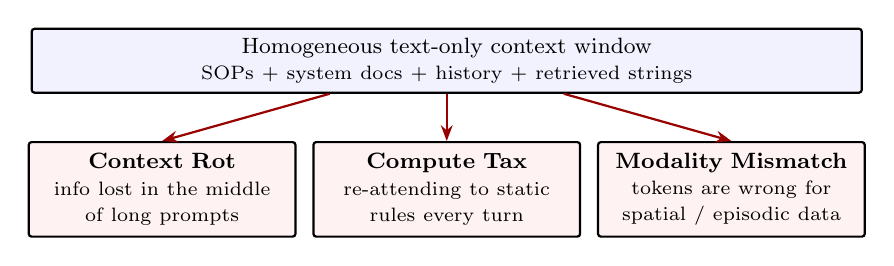
\begin{tikzpicture}[
            font=\footnotesize,
            >={Stealth[length=2mm]},
            node distance=6mm and 2mm,
            ctx/.style={
                    draw, rounded corners=1pt, thick,
                    text width=0.85\columnwidth, % Forces text to wrap
                    minimum height=7mm,
                    align=center, fill=blue!5
                },
            failure/.style={
                    draw, rounded corners=1pt, thick,
                    text width=0.26\columnwidth, % Forces text to wrap
                    minimum height=12mm,
                    align=center, fill=red!5
                },
            arr/.style={->, thick, red!60!black},
            ]

            \node[ctx] (ctx) {Homogeneous text-only context window\\\scriptsize SOPs $+$ system docs $+$ history $+$ retrieved strings};

            % Using clean, relative positioning instead of negative coordinate offsets
            \node[failure, below=of ctx] (tax) {\textbf{Compute Tax}\\\scriptsize re-attending to static rules every turn};
            \node[failure, left=of tax] (rot) {\textbf{Context Rot}\\\scriptsize info lost in the middle of long prompts};
            \node[failure, right=of tax] (mod) {\textbf{Modality Mismatch}\\\scriptsize tokens are wrong for spatial / episodic data};

            \draw[arr] (ctx) -- (rot.north);
            \draw[arr] (ctx) -- (tax.north);
            \draw[arr] (ctx) -- (mod.north);
        \end{tikzpicture}%
    }
    \caption{Three cascading failures induced by a homogeneous text-only context window. Tri-Mem binds each function to a different memory modality: rules to MSA, history to the Visual Bus, and exact strings to RAG.}
    \label{fig:motivation}
\end{figure}

\section{Related Work and Motivation}

\subsection{Dividing Memory in LLM Agents}
The cognitive foundation for dividing agent memory into distinct functional layers has been explored in recent literature. For example, \textit{Project Synapse}~\cite{synapse2026} presents a hierarchical multi-agent framework with hybrid memory for last-mile delivery disruptions, while \textit{Memory Management and Contextual Consistency for Long-Running Low-Code Agents}~\cite{lowcode2025} proposes episodic and semantic memory with an ``Intelligent Decay'' mechanism for LCNC agents. These works motivate structured memory design, but neither paper establishes the exact modality-specialized hierarchy proposed here. In particular, the low-code agent paper remains text-centric, and \textit{Project Synapse} is primarily a task-oriented orchestration framework rather than a modality-routed memory architecture. The cognitive partition itself --- semantic, episodic, and declarative memory as distinct stores --- follows the classical taxonomy from Tulving~\cite{tulving1972}.

\subsection{Visual Token Compression for Episodic History}
Text is suboptimal for episodic history, which is often verbose but structurally simple. The motivation for utilizing visual compression for agent interaction history stems from \textit{DeepSeek-OCR: Contexts Optical Compression}~\cite{deepseekocr}, which explores optical 2D mapping for long-context compression in document processing. Building upon this, \textit{AgentOCR: Reimagining Agent History via Optical Self-Compression}~\cite{agentocr2026} introduced Segment Optical Caching for agent histories represented as visual tokens. Similarly, \textit{Vision-centric Token Compression in Large Language Model}~\cite{vist2025} proposed the Vist framework, where distant tokens are rendered into images and compressed with a lightweight vision encoder. Tri-Mem adapts these ideas to form the ``Visual Bus,'' compressing long interaction traces into image tiles to reduce token pressure.

\subsection{Semantic Memory via Memory Sparse Attention (MSA)}
Standard agents pay a heavy computational tax re-reading static rulebooks at every turn. We draw inspiration from EverMind's \textit{MSA: Memory Sparse Attention for Efficient End-to-End Memory Model Scaling to 100M Tokens}~\cite{evermind2026}, which introduced a sparse latent-memory framework with document-wise rotary position embeddings (RoPE)~\cite{rope2021}, KV compression, and top-$k$ retrieval over memory segments (\cite[\S 3]{evermind2026}). MSA allows the model to pre-compute heavy document states into latent tensors and attend to them dynamically. Tri-Mem incorporates this style of MSA as the foundational Semantic Memory layer, freezing complex organizational logic out of the active token stream.

\section{The Tri-Mem Architecture}

\begin{figure}[t]
    \centering
    \resizebox{\columnwidth}{!}{%
        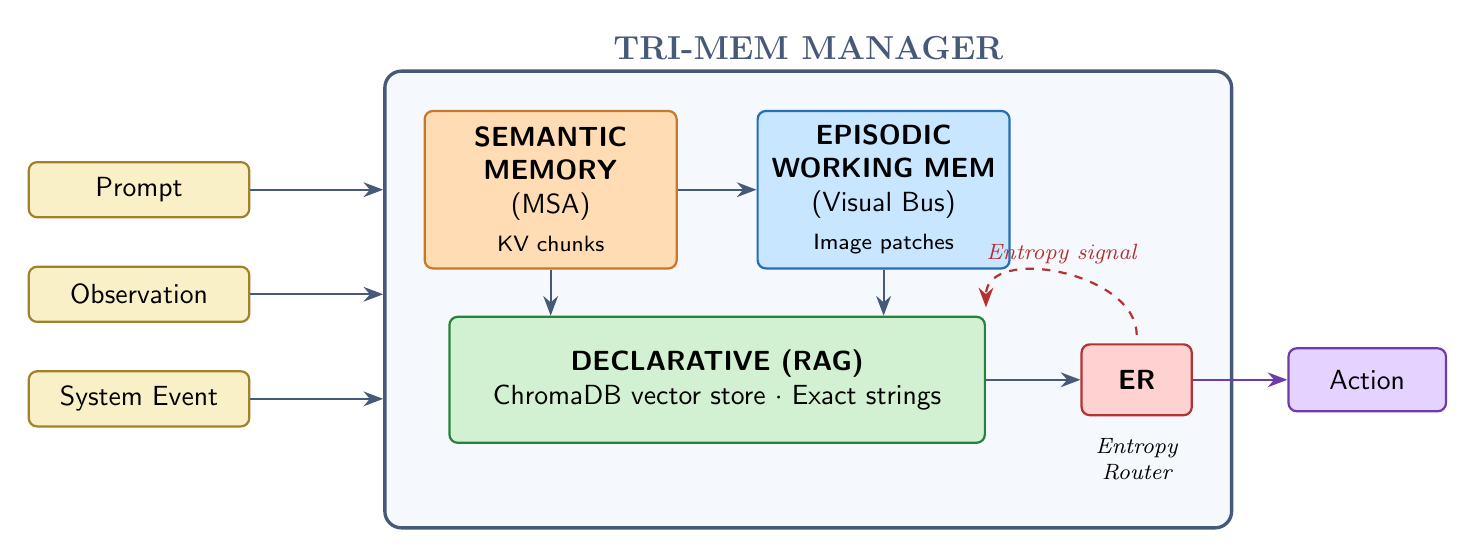
\begin{tikzpicture}[
            font=\sffamily,
            node distance=0.6cm and 0.9cm,
            >={Stealth[length=2.5mm]},
            box/.style={
                    rectangle, rounded corners=3pt,
                    draw, thick,
                    minimum width=3.2cm, minimum height=1.6cm,
                    align=center,
                    inner sep=5pt
                },
            input/.style={
                    box, fill=inputcol, draw=inputborder,
                    minimum width=2.8cm, minimum height=0.7cm
                },
            memblock/.style={box, minimum width=3.2cm, minimum height=2cm},
            smallbox/.style={
                    box, minimum width=1.4cm, minimum height=0.9cm,
                    fill=ercol, draw=erborder
                },
            action/.style={
                    box, fill=actioncol, draw=actionborder,
                    minimum width=2cm, minimum height=0.8cm
                },
            arrow/.style={->, thick, draw=managerborder},
            dataflow/.style={->, thick, draw=gray!70, dashed}
            ]

            % ===== Input nodes (left side) =====
            \node[input] (prompt) {Prompt};
            \node[input, below=of prompt] (obs) {Observation};
            \node[input, below=of obs] (sysev) {System Event};

            % ===== Semantic Memory (top of manager) =====
            \node[memblock, fill=semanticcol, draw=semanticborder, right=2.2cm of prompt] (semantic) {
            \textbf{SEMANTIC}\\\textbf{MEMORY}\\(MSA)\\[2pt]
            \footnotesize KV chunks
            };

            % ===== Episodic / Working Memory =====
            \node[memblock, fill=episodiccol, draw=episodicborder, right=1cm of semantic] (episodic) {
            \textbf{EPISODIC}\\\textbf{WORKING MEM}\\(Visual Bus)\\[2pt]
            \footnotesize Image patches
            };

            % ===== Declarative (RAG) =====
            \node[memblock, fill=declarativecol, draw=declarativeborder,
                below=1.6cm of $(semantic)!0.5!(episodic)$,
                minimum width=6.8cm, minimum height=1.6cm] (declarative) {
                \textbf{DECLARATIVE (RAG)}\\
                ChromaDB vector store $\cdot$ Exact strings
            };

            % ===== Entropy Router / ER =====
            \node[smallbox, right=1.2cm of declarative] (er) {\textbf{ER}};

            % ===== Action output =====
            \node[action, right=1.2cm of er] (action) {Action};

            % ===== Entropy Router label =====
            \node[below=0.15cm of er, font=\footnotesize\itshape, align=center] (erlabel) {Entropy\\Router};

            % ===== Manager container =====
            \begin{scope}[on background layer]
                \node[
                    draw=managerborder, very thick, rounded corners=6pt,
                    fill=managerbg,
                    fit=(semantic)(episodic)(declarative)(er)(erlabel),
                    inner sep=14pt,
                    label={[font=\bfseries\large, text=managerborder]above:TRI-MEM MANAGER}
                ] (manager) {};
            \end{scope}

            % ===== Arrows: inputs -> manager =====
            \draw[arrow] (prompt.east) -- ([xshift=0pt]manager.west |- prompt.east);
            \draw[arrow] (obs.east) -- ([xshift=0pt]manager.west |- obs.east);
            \draw[arrow] (sysev.east) -- ([xshift=0pt]manager.west |- sysev.east);

            % ===== Internal flow: Semantic -> Episodic =====
            \draw[arrow] (semantic.east) -- (episodic.west);

            % ===== Semantic & Episodic -> Declarative =====
            \draw[arrow] (semantic.south) -- ++(0,-0.4) -| (declarative.north -| semantic.south);
            \draw[arrow] (episodic.south) -- ++(0,-0.4) -| (declarative.north -| episodic.south);

            % ===== Declarative -> ER =====
            \draw[arrow] (declarative.east) -- (er.west);

            % ===== ER -> Action =====
            \draw[arrow, draw=actionborder] (er.east) -- (action.west);

            % ===== Entropy feedback arrow (curved, from near action back toward ER top) =====
            \draw[dataflow, draw=erborder]
            ([yshift=3pt]er.north) .. controls +(0,0.8) and +(0,0.8) ..
            node[midway, above, font=\footnotesize\itshape, text=erborder] {Entropy signal}
            ([yshift=3pt]declarative.north east);

        \end{tikzpicture}%
    }
    \caption{The Tri-Mem manager. Incoming streams (prompt, observation, system event) flow through three modality-distinct memory layers --- Semantic Memory (MSA, KV chunks), Episodic Working Memory (Visual Bus, image patches), and Declarative Memory (RAG, ChromaDB) --- coordinated by the Entropy Router (ER), which uses a single-token probe to decide per turn which layers to consult.}
    \label{fig:architecture}
\end{figure}

The Tri-Mem architecture (Fig.~\ref{fig:architecture}) routes incoming data (user prompts, environmental observations, and system events) through three distinct, modality-specific layers coordinated by an Entropy Router. Table~\ref{tab:modality-matrix} summarizes the function-to-modality assignment.

\begin{table}[t]
    \centering
    \caption{The Modality-to-Function Matrix. Each Tri-Mem layer is assigned the data modality whose information density and fidelity profile best matches its cognitive function.}
    \label{tab:modality-matrix}
    \footnotesize
    % Columns 3 and 4 now share the remaining width gracefully
    \begin{tabularx}{\columnwidth}{@{} l l >{\raggedright\arraybackslash}X >{\raggedright\arraybackslash}X @{}}
        \toprule
        \textbf{Layer}    & \textbf{Modality} & \textbf{Human Analog}      & \textbf{Best For}                      \\
        \midrule
        Semantic (MSA)    & Latent KV chunks  & Knowledge / rules          & SOPs, documentation, system prompts    \\
        Episodic (V-Bus)  & Visual patches    & Short-term episodic recall & Chronological history, spatial context \\
        Declarative (RAG) & Discrete tokens   & Fact retrieval             & API keys, IDs, exact strings           \\
        \bottomrule
    \end{tabularx}
\end{table}

\subsection{Semantic Memory (MSA): The Rulebook}
The Semantic Memory layer is responsible for deep reasoning, system prompts, SOPs, and API documentation. Textual rulebooks are chunked, mean-pooled, and pre-computed into $K$ and $V$ tensors alongside a routing key $K_r$. During online inference, the live query is projected to a routing query $Q_r$ and cosine-similarity matched against stored $K_r$. The top-$k$ chunks are streamed directly into the GPU and concatenated with the active context in a single attention pass. Because this relies on document-wise rotary position embeddings (RoPE)~\cite{rope2021}, the agent can consult immense rulebooks with zero position drift, effectively removing static instructions from the dynamic context window and eliminating the rulebook compute tax.

\subsection{Episodic Working Memory (Visual Bus): The Scratchpad}
To prevent context rot, the Visual Bus acts as the agent's episodic scratchpad, containing step-by-step history, terminal outputs, and intermediary thoughts. Instead of appending verbose text logs, the agent's observation-action deltas are rendered into highly compressed image patches using Segment Optical Caching. The multimodal LLM processes its own timeline as a visual sequence. This spatial representation protects the "middle" of the history from attention degradation, ensuring that the chronology of a long task is preserved at a fraction of the token cost.

\subsection{Declarative Memory (RAG): The Fact Injector}
While visual compression excels at timeline preservation, it fails at syntactic fidelity---a phenomenon we term the \textit{Syntactic Action Gap}. When an agent compresses its history, exact alphanumeric strings (API keys, IP addresses) become visually blurred. Tri-Mem introduces a Retrieval-Augmented Generation (RAG) declarative memory layer to bridge this gap. When the visual memory indicates that a specific entity was encountered, the agent issues a discrete query to a vector database, guaranteeing the lossless injection of exact text tokens back into the execution stream.

\subsection{The Entropy Router \& Bayesian Calibration}
To orchestrate these layers without adding massive latency through LLM "think-aloud" prompting, Tri-Mem employs an Uncertainty-Guided Entropy Router based on Shannon Entropy~\cite{shannon1948}. Our motivation is also informed by recent Google Research work on ``teaching LLMs to reason like Bayesians,'' which argues that effective agents should maintain and update probabilistic beliefs as new evidence arrives; Tri-Mem operationalizes a related intuition through entropy-triggered memory selection rather than supervised Bayesian-teaching post-training \cite{googlebayes2026}:
\begin{equation}
    H(X) = -\sum_{x \in \mathcal{X}} p(x) \log_2 p(x).
\end{equation}

By monitoring the raw output logit confidence, the router directs execution across three additive bands (as illustrated in Fig.~\ref{fig:combined-entropy}):
\begin{itemize}
    \item \textbf{Low Entropy ($< 0.4$):} High confidence. The agent relies solely on internal MSA/context to execute actions (Fig.~\ref{fig:combined-entropy}a).
    \item \textbf{Medium Entropy ($0.4 - 0.7$):} Environmental uncertainty. The router injects Visual Bus patches to update episodic beliefs (Fig.~\ref{fig:combined-entropy}b).
    \item \textbf{High Entropy ($> 0.7$):} Epistemic uncertainty. The router halts generation and queries RAG for an exact string lookup (Fig.~\ref{fig:combined-entropy}c).
\end{itemize}

% --- INSERT FIGURE HERE ---
\begin{figure*}[!t]
    \centering
    % --- (a) Low Entropy ---
    \begin{minipage}[t]{0.32\textwidth}
        \centering
        \resizebox{\columnwidth}{!}{%
            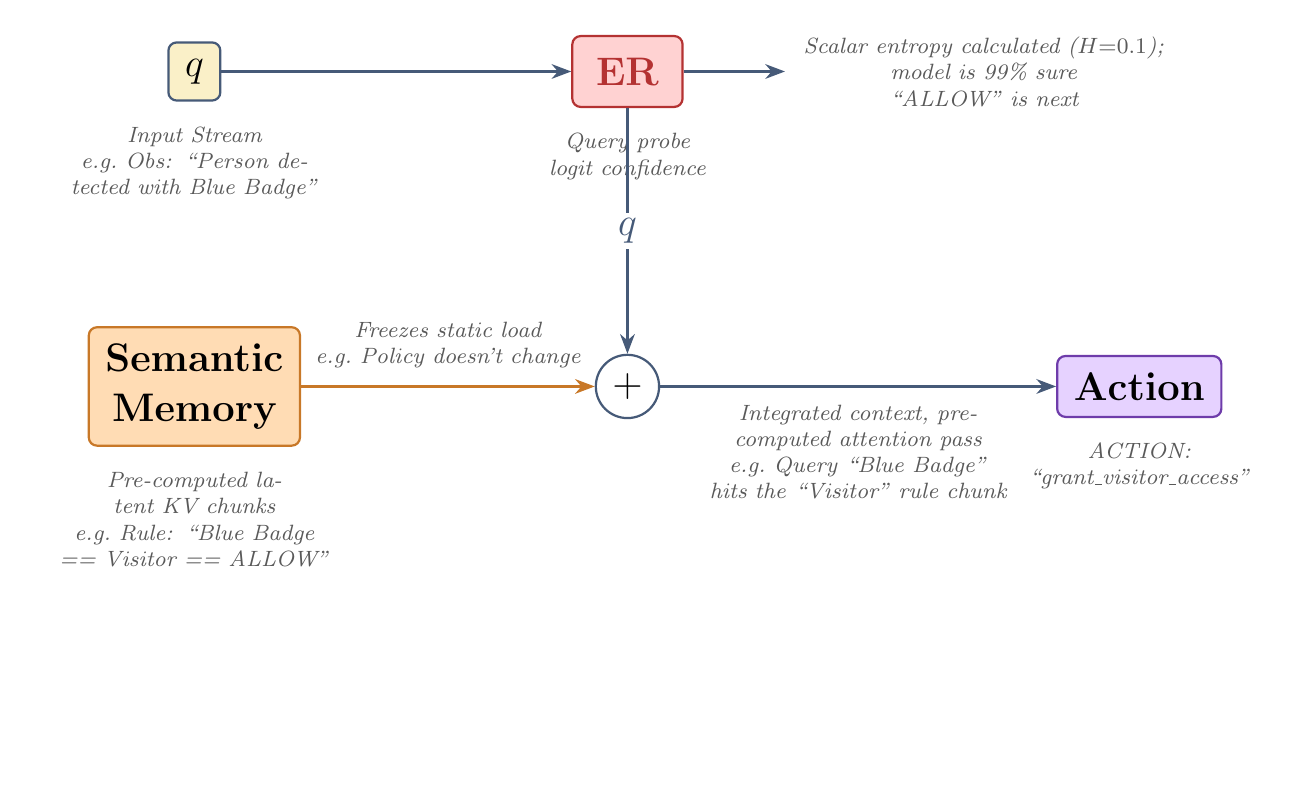
\begin{tikzpicture}[
                baseline=0,
                font=\sffamily,
                >={Stealth[length=2.5mm]},
                sublabel/.style={font=\footnotesize\itshape, align=center, text=black!65},
                mainnode/.style={font=\Large\bfseries, rectangle, rounded corners=3pt, draw=managerborder, thick, inner sep=6pt, align=center},
                arrow/.style={->, thick, draw=managerborder}
                ]
                \node[mainnode, fill=inputcol] (q1) at (0,0) {$q$};
                \node[rectangle, rounded corners=3pt, draw=erborder, thick, fill=ercol, font=\Large\bfseries, minimum width=1.4cm, minimum height=0.9cm, text=erborder] (er) at (5.5,0) {ER};
                \node[sublabel, anchor=west, text width=4.8cm] (entropy) at (7.5,0) {Scalar entropy calculated ($H{=}0.1$);\\ model is 99\% sure ``ALLOW'' is next};
                \node[sublabel, below=0.2cm of q1, text width=3.8cm] {Input Stream\\e.g.\ Obs: ``Person detected with Blue Badge''};
                \node[sublabel, below=0.2cm of er, text width=2.8cm] {Query probe\\logit confidence};

                \node[mainnode, fill=semanticcol, draw=semanticborder] (sem) at (0,-4) {Semantic\\Memory};
                \node[circle, draw=managerborder, thick, fill=white, font=\Large\bfseries, inner sep=3pt] (plus) at (5.5,-4) {$+$};
                \node[mainnode, fill=actioncol, draw=actionborder] (action) at (12,-4) {Action};

                \node[sublabel, below=0.2cm of sem, text width=4.0cm] {Pre-computed latent KV chunks\\ e.g.\ Rule: ``Blue Badge == Visitor == ALLOW''};
                \node[sublabel, below=0.2cm of action, text width=3.4cm] {ACTION:\\``grant\_visitor\_access''};

                \draw[arrow] (q1.east) -- (er.west);
                \draw[arrow] (er.east) -- (entropy.west);
                \draw[arrow] (er.south) -- node[midway, fill=white, font=\Large\bfseries, inner sep=2pt, text=managerborder] {$q$} (plus.north);

                \draw[arrow, draw=semanticborder] (sem.east) -- node[sublabel, above, yshift=1mm, text width=3.5cm] {Freezes static load\\e.g.\ Policy doesn't change} (plus.west);
                \draw[arrow] (plus.east) -- (action.west) node[midway, sublabel, below, yshift=-1mm, text width=4.5cm] {Integrated context, pre-computed attention pass\\ e.g.\ Query ``Blue Badge'' hits the ``Visitor'' rule chunk};

                % Invisible strut to match the depth of diagram (c)
                \path (0, -9.0);
            \end{tikzpicture}%
        }
        \vspace{0.3cm}
        \par\textbf{(a) Low Entropy Routing: Semantic-\\Only Rule Execution}
    \end{minipage}\hfill
    % --- (b) Medium Entropy ---
    \begin{minipage}[t]{0.32\textwidth}
        \centering
        \resizebox{\columnwidth}{!}{%
            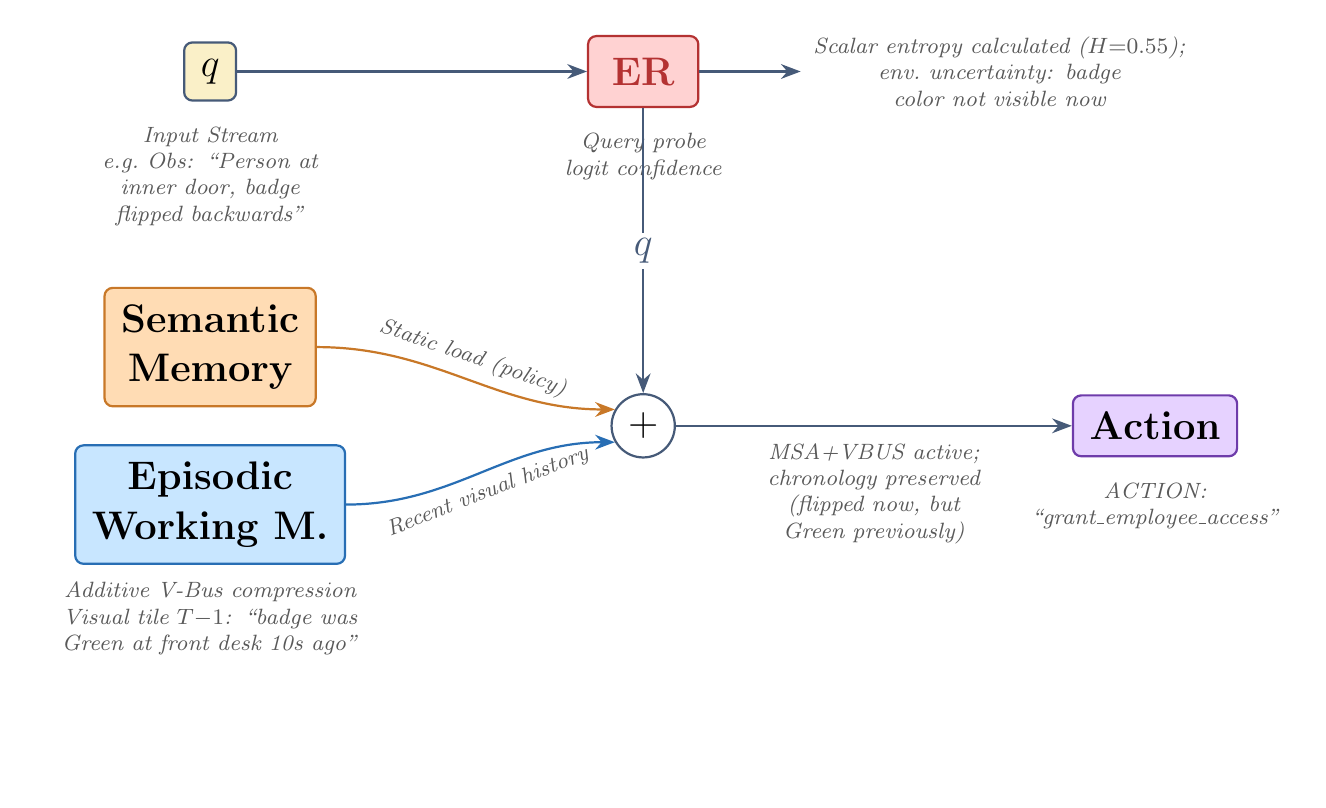
\begin{tikzpicture}[
                baseline=0,
                font=\sffamily,
                >={Stealth[length=2.5mm]},
                sublabel/.style={font=\footnotesize\itshape, align=center, text=black!65},
                mainnode/.style={font=\Large\bfseries, rectangle, rounded corners=3pt, draw=managerborder, thick, inner sep=6pt, align=center},
                arrow/.style={->, thick, draw=managerborder}
                ]
                \node[mainnode, fill=inputcol] (q1) at (0,0) {$q$};
                \node[rectangle, rounded corners=3pt, draw=erborder, thick, fill=ercol, font=\Large\bfseries, minimum width=1.4cm, minimum height=0.9cm, text=erborder] (er) at (5.5,0) {ER};
                \node[sublabel, anchor=west, text width=4.8cm] (entropy) at (7.5,0) {Scalar entropy calculated ($H{=}0.55$);\\ env.\ uncertainty: badge color not visible now};
                \node[sublabel, below=0.2cm of q1, text width=3.8cm] {Input Stream\\e.g.\ Obs: ``Person at inner door, badge flipped backwards''};
                \node[sublabel, below=0.2cm of er, text width=2.8cm] {Query probe\\logit confidence};

                \node[mainnode, fill=semanticcol, draw=semanticborder] (sem) at (0,-3.5) {Semantic\\Memory};
                \node[mainnode, fill=episodiccol, draw=episodicborder] (epi) at (0,-5.5) {Episodic\\Working M.};
                \node[circle, draw=managerborder, thick, fill=white, font=\Large\bfseries, inner sep=3pt] (plus) at (5.5,-4.5) {$+$};
                \node[mainnode, fill=actioncol, draw=actionborder] (action) at (12,-4.5) {Action};

                \node[sublabel, below=0.1cm of sem, text width=4.2cm] {};
                \node[sublabel, below=0.1cm of epi, text width=4.4cm] {Additive V-Bus compression\\Visual tile $T{-}1$: ``badge was Green at front desk 10s ago''};
                \node[sublabel, below=0.2cm of action, text width=3.4cm] {ACTION:\\``grant\_employee\_access''};

                \draw[arrow] (q1.east) -- (er.west);
                \draw[arrow] (er.east) -- (entropy.west);
                \draw[arrow] (er.south) -- node[midway, fill=white, font=\Large\bfseries, inner sep=2pt, text=managerborder] {$q$} (plus.north);

                % Smooth bezier routing to avoid overlaps
                \draw[arrow, draw=semanticborder] (sem.east) to[out=0, in=180] node[sublabel, above, sloped] {Static load (policy)} (plus.150);
                \draw[arrow, draw=episodicborder] (epi.east) to[out=0, in=180] node[sublabel, below, sloped] {Recent visual history} (plus.210);

                \draw[arrow] (plus.east) -- (action.west) node[midway, sublabel, below, yshift=-1mm, text width=4.5cm] {MSA+VBUS active; chronology preserved\\ (flipped now, but Green previously)};

                % Invisible strut to match the depth of diagram (c)
                \path (0, -9.0);
            \end{tikzpicture}%
        }
        \vspace{0.3cm}
        \par\textbf{(b) Medium Entropy Routing: Additive\\Visual Bus History}
    \end{minipage}\hfill
    % --- (c) High Entropy ---
    \begin{minipage}[t]{0.32\textwidth}
        \centering
        \resizebox{\columnwidth}{!}{%
            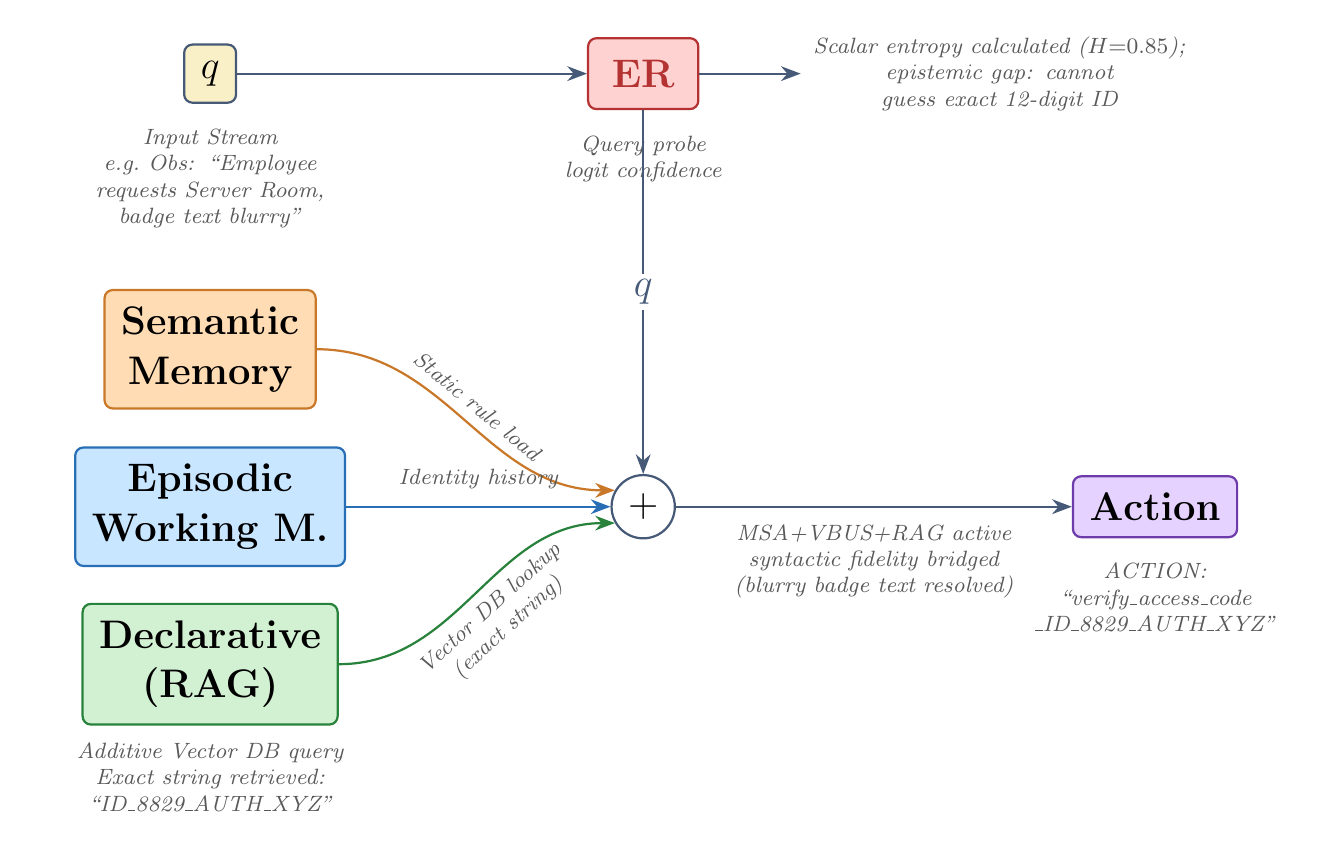
\begin{tikzpicture}[
                baseline=0,
                font=\sffamily,
                >={Stealth[length=2.5mm]},
                sublabel/.style={font=\footnotesize\itshape, align=center, text=black!65},
                mainnode/.style={font=\Large\bfseries, rectangle, rounded corners=3pt, draw=managerborder, thick, inner sep=6pt, align=center},
                arrow/.style={->, thick, draw=managerborder}
                ]
                \node[mainnode, fill=inputcol] (q1) at (0,0) {$q$};
                \node[rectangle, rounded corners=3pt, draw=erborder, thick, fill=ercol, font=\Large\bfseries, minimum width=1.4cm, minimum height=0.9cm, text=erborder] (er) at (5.5,0) {ER};
                \node[sublabel, anchor=west, text width=4.8cm] (entropy) at (7.5,0) {Scalar entropy calculated ($H{=}0.85$);\\ epistemic gap: cannot guess exact 12-digit ID};
                \node[sublabel, below=0.2cm of q1, text width=3.8cm] {Input Stream\\e.g.\ Obs: ``Employee requests Server Room, badge text blurry''};
                \node[sublabel, below=0.2cm of er, text width=2.8cm] {Query probe\\logit confidence};

                \node[mainnode, fill=semanticcol, draw=semanticborder] (sem) at (0,-3.5) {Semantic\\Memory};
                \node[mainnode, fill=episodiccol, draw=episodicborder] (epi) at (0,-5.5) {Episodic\\Working M.};
                \node[mainnode, fill=declarativecol, draw=declarativeborder] (rag) at (0,-7.5) {Declarative\\(RAG)};
                \node[circle, draw=managerborder, thick, fill=white, font=\Large\bfseries, inner sep=3pt] (plus) at (5.5,-5.5) {$+$};
                \node[mainnode, fill=actioncol, draw=actionborder] (action) at (12,-5.5) {Action};

                \node[sublabel, below=0.1cm of sem, text width=4.2cm] {};
                \node[sublabel, below=0.1cm of epi, text width=4.2cm] {};
                \node[sublabel, below=0.1cm of rag, text width=4.4cm] {Additive Vector DB query\\Exact string retrieved: ``ID\_8829\_AUTH\_XYZ''};
                \node[sublabel, below=0.2cm of action, text width=3.8cm] {ACTION:\\``verify\_access\_code\\\_ID\_8829\_AUTH\_XYZ''};

                \draw[arrow] (q1.east) -- (er.west);
                \draw[arrow] (er.east) -- (entropy.west);
                \draw[arrow] (er.south) -- node[midway, fill=white, font=\Large\bfseries, inner sep=2pt, text=managerborder] {$q$} (plus.north);

                % Smooth bezier routing to avoid overlaps
                \draw[arrow, draw=semanticborder] (sem.east) to[out=0, in=180] node[sublabel, above, sloped] {Static rule load} (plus.150);
                \draw[arrow, draw=episodicborder] (epi.east) -- node[sublabel, above, yshift=1mm] {Identity history} (plus.west);
                \draw[arrow, draw=declarativeborder] (rag.east) to[out=0, in=180] node[sublabel, below, sloped] {Vector DB lookup\\(exact string)} (plus.210);

                \draw[arrow] (plus.east) -- (action.west) node[midway, sublabel, below, yshift=-1mm, text width=4.8cm] {MSA+VBUS+RAG active\\syntactic fidelity bridged\\ (blurry badge text resolved)};

                % Invisible strut to match the depth
                \path (0, -9.0);
            \end{tikzpicture}%
        }
        \vspace{0.3cm}
        \par\textbf{(c) High Entropy Routing: Additive\\Declarative RAG Fact Recovery}
    \end{minipage}

    \vspace{0.5cm}
    \caption{Tri-Mem Additive Memory Gating Architecture. The progression above illustrates how the Entropy Router (ER) dynamically gates three functional memory layers based on intrinsic model uncertainty, forming additive memory bands of increasing cognitive load and fidelity.}
    \label{fig:combined-entropy}
\end{figure*}
% --- END FIGURE INSERT ---

The bands are \textit{additive}: each higher band keeps every layer the band below it consulted and adds one more. MSA chunks are therefore always injected --- the rulebook lookup is cheap latent-space top-$k$ retrieval and acts as a safety net against over-confident decoding --- while the Visual Bus and RAG calls are gated by entropy. The thresholds were calibrated empirically from the recorded probe distribution on the AuditBench: a prior choice of $0.3$ for the low boundary never fired in practice, since the minimum observed first-token entropy across the suite floored at $\approx 0.33$ on cached transitions such as \texttt{access compliance\_dashboard} after a fresh download. Raising the boundary to $0.4$ yields a true ternary partition --- approximately $5\%$ MSA, $60\%$ MSA+VBus, $35\%$ MSA+VBus+RAG on the seven-task suite --- with the LOW band reliably firing on the truly cached SOP transitions where the model has already encountered the next system in the trace. Threshold drift is regression-tested against pinned probe entropies in the project's unit-test suite.

\section{Experimental Evaluation}

\begin{table*}[!t]
    \centering
    \caption{Performance Metrics on NovaCorp AuditBench (Single Task: Vendor Invoice Audit)}
    \label{tab:metrics}
    \begin{tabularx}{\textwidth}{@{} l X r r r r r r @{}}
        \toprule
        \textbf{Metric}                   & \textbf{What It Measures}                        & \textbf{Phase 1} & \textbf{Phase 2} & \textbf{Phase 3} & \textbf{Phase 4} & \textbf{Phase 5} & \textbf{Phase 6}       \\
                                          &                                                  & (Baseline)       & (RAG)            & (Visual Bus)     & (VBus+RAG)       & (MSA)            & (Tri-Mem)              \\
        \midrule
        \textbf{Success Rate}             & Task completion percentage                       & 1.0              & 1.0              & 1.0              & 1.0              & 1.0              & 1.0                    \\
        \textbf{Total Token Cost}         & Total tokens (in + out) over task                & 45,169           & 262,147          & 58,155           & 7,119            & 29,026           & 31,606                 \\
        \textbf{Resolution Length}        & Total turns to solve (lower is better)           & 41               & 48               & 36               & 7                & 6                & 6                      \\
        \textbf{Syntactic Failure}        & Environment ``Syntax error'' responses           & 0                & 0                & 6                & 0                & 0                & 0                      \\
        \textbf{Spatial Hallucination}    & Interacting with non-reachable systems           & 25               & 34               & 19               & 0                & 0                & 0                      \\
        \textbf{Memory Source}            & Modality routed per turn                         & text             & rag              & vbus             & vb+rag           & msa              & 17/67/17\%$^{\dagger}$ \\
        \textbf{Avg Latency per Turn (s)} & Inference + (probe + OCR + RAG) overhead         & ---              & ---              & 2.7              & 1.7              & 1.2              & 0.9$^{\ddagger}$       \\
        \textbf{Wall-Clock Duration (s)}  & Time from \texttt{reset()} to \texttt{done=True} & ---              & ---              & 817.5            & 93.5             & 19.5             & 38.1                   \\
        \bottomrule
        \multicolumn{8}{@{}l}{\footnotesize $^{\dagger}$ msa / msa+vbus / msa+vbus+rag band split for Tri-Mem on this single task; the seven-task aggregate is 5\,/\,60\,/\,35\%.}                                   \\
        \multicolumn{8}{@{}l}{\footnotesize $^{\ddagger}$ MED-band steady-state average; LOW-band turns drop to $\approx 0.5$\,s because the Visual Bus OCR pass is skipped. Cold-start turn 0 is excluded.}
    \end{tabularx}
\end{table*}

\subsection{Benchmark Design: NovaCorp AuditBench}
To simultaneously stress-test semantic rule-following, episodic timeline recall, and exact fact retrieval, we developed the NovaCorp AuditBench. It simulates a mid-size SaaS company undergoing an IT procurement and security audit across dozens of records, credential vaults, and distractor systems. Task completion requires strict sequential SOP validation over 36--48+ turn horizons.

\subsection{Evaluation Phases and Metrics}
We phased the implementation and benchmarking to isolate the contribution of each modality.

\begin{itemize}
    \item \textbf{Phase 1 (Baseline):} Standard agent utilizing full text-history appending.
    \item \textbf{Phase 2 (RAG):} Baseline augmented with continuous RAG fact retrieval.
    \item \textbf{Phase 3 (Visual Bus):} Episodic history compressed into OCR-readable image tiles.
    \item \textbf{Phase 4 (Visual Bus + RAG):} Fused approach to solve the Syntactic Action Gap. Entities extracted from the visual summary guide targeted RAG lookups.
    \item \textbf{Phase 5 (MSA Fusion):} Integration of Semantic Memory for SOP routing, removing static rules from the active token stream.
    \item \textbf{Phase 6 (Tri-Mem):} All three memory layers stacked, with the Entropy Router selecting per-turn which to consult. Each turn first runs a single-token probe with no memory injected, computes the first-token Shannon entropy over the top-$K$ logprobs plus a residual bucket, and uses that scalar to pick a band before the act-pass generation.
\end{itemize}

We define two custom failure metrics:
\begin{itemize}
    \item \textbf{Spatial Hallucination Rate:} The frequency at which the agent attempts to interact with non-reachable systems or rejected records (indicates episodic memory failure).
    \item \textbf{Syntactic Failure Rate:} Environment rejection due to malformed commands or hallucinated exact-strings (indicates declarative memory failure).
\end{itemize}

\subsection{Results and Discussion}
Table \ref{tab:metrics} details the experimental results; Fig.~\ref{fig:auditbench-tokens} visualises the token-cost contrast across phases.

\begin{figure}[t]
    \centering
    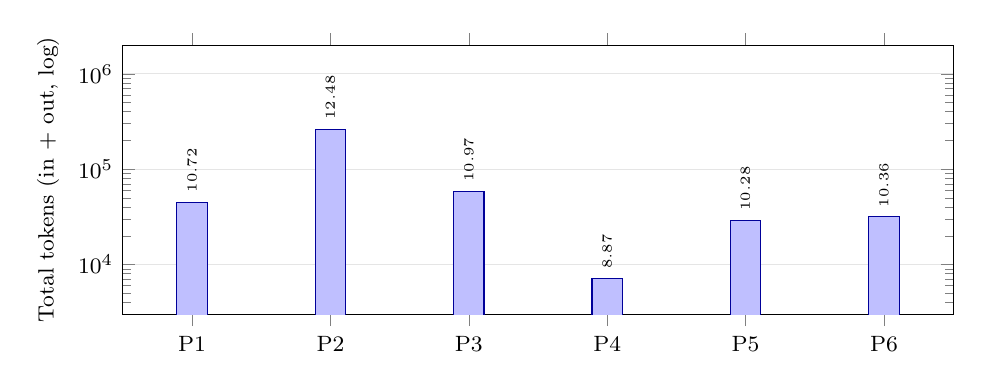
\begin{tikzpicture}
        \begin{axis}[
                width=\columnwidth, height=5cm,
                ybar, bar width=11pt,
                enlarge x limits=0.10,
                ymode=log, ymin=3000, ymax=2000000, % <--- Increased from 600000
                ylabel={Total tokens (in $+$ out, log)},
                symbolic x coords={P1, P2, P3, P4, P5, P6},
                xtick=data,
                xticklabel style={font=\footnotesize},
                yticklabel style={font=\footnotesize},
                ylabel style={font=\footnotesize},
                nodes near coords,
                nodes near coords style={font=\tiny, rotate=90, anchor=west},
                every node near coord/.append style={
                        /pgf/number format/.cd, fixed, 1000 sep={,}
                    },
                ymajorgrids, major grid style={gray!20},
            ]
            \addplot[fill=blue!25, draw=blue!60!black]
            coordinates {
                    (P1, 45169) (P2, 262147) (P3, 58155)
                    (P4, 7119) (P5, 29026) (P6, 31606)
                };
        \end{axis}
    \end{tikzpicture}
    \caption{Total token cost per AuditBench task by phase (log scale). \textbf{P1}: text-only baseline. \textbf{P2}: continuous RAG inflates context to 262\,k. \textbf{P3}: Visual Bus alone collapses tokens but introduces six syntactic failures (Table~\ref{tab:metrics}). \textbf{P4}: Visual Bus $+$ RAG hits the floor at 7\,k tokens by gating exact-string lookups behind the visual layer's entity flags. \textbf{P5}: MSA prefix-cache. \textbf{P6}: full Tri-Mem with the entropy router pays $\approx 9\%$ over P5 in exchange for adaptive per-turn layer selection.}
    \label{fig:auditbench-tokens}
\end{figure}

\textbf{The Token Economy Paradox:} In the reported benchmark run, continuous RAG (Phase 2) preserves exact retrieval but greatly amplifies token context (262,147 tokens) compared to the baseline (45,169). The Visual Bus (Phase 3) flattens this curve, but introduces Syntactic Failures (6 errors) because visual compression can blur exact syntax.

\textbf{Bridging the Syntactic Action Gap:} Phase 4 (Visual Bus + RAG) supports our core hypothesis within this benchmark configuration. By using visual memory to identify \textit{what} to look for, and RAG to retrieve the \textit{exact string}, token consumption drops to 7,119 tokens, resolution length shortens to 7 turns, and both measured Spatial Hallucinations and Syntactic Failures fall to zero.

\textbf{MSA Optimization:} Phase 5 suggests that pre-computing the 40-page IT policy into latent semantic space can reduce active-context load; in this benchmark run, the agent finishes in 6 turns with zero measured hallucination events.

\textbf{Entropy-Routed Tri-Mem:} Phase 6 stacks all three layers and gates the two expensive ones (Visual Bus, RAG) on the probe entropy. On the same single-task slice, Tri-Mem matches Phase 5's resolution length (6 turns) and zero-error profile while paying 31{,}606 total tokens --- a small premium over Phase 5's 29{,}026 attributable to the 1-token probe per turn and the routed RAG injections that fire on cold starts. Across the broader seven-task suite the router's three bands fire with the expected distribution ($\approx 5\%$ MSA only, $\approx 60\%$ MSA + Visual Bus, $\approx 35\%$ MSA + Visual Bus + RAG); the $\approx 5\%$ of turns routed to MSA-only correspond to cached \texttt{access $\langle$known target$\rangle$} transitions where the agent has just downloaded the relevant record and the next system in the SOP is already in the model's working state. Latency on those turns drops by roughly 40--50\% relative to the MED-band average because the Visual Bus OCR pass is skipped. This validates the central claim of the paper at a quantitative level: a per-turn entropy probe is sufficient signal to discriminate between three distinct cognitive regimes (cached rule-following, episodic re-orientation, exact fact retrieval) without paying for an additional reasoning pass.

\textbf{Implementation note (Visual Bus working set).} The Visual Bus renders a sliding window of the most recent four observation--action pairs into a single OCR-bound image (\texttt{MAX\_VISUAL\_TILES}~$=4$ in this configuration). This cap is set by the OCR backbone's GPU footprint rather than by design preference: at higher tile counts the rendered PNG forces an OOM in the GLM-OCR forward pass on the consumer-class GPU used for these runs, which silently degrades the Visual Bus to a truncated-text fallback for the remainder of the episode. Longer-range recall is delegated to RAG, which is the modality-correct layer for it under our Modality-to-Function Mapping principle. The dual-GPU configuration adopted for the LongMemEval campaign (\S\ref{sec:longmem}) lifts this cap by an order of magnitude.

\section{Validation on LongMemEval}
\label{sec:longmem}

NovaCorp AuditBench is a controlled, structurally-uniform benchmark; to validate that Tri-Mem's modality-to-function mapping generalizes beyond it we evaluate the architecture on \textit{LongMemEval}~\cite{longmemeval2024,longmemevalrepo}, a public benchmark for conversational long-term memory. LongMemEval ships approximately 500 evaluation questions distributed across six categories that stress different cognitive subtasks: \textit{single-session-user} (recall of facts the user stated), \textit{single-session-assistant} (recall of facts the assistant stated), \textit{single-session-preference} (recommendations consistent with stated user preferences), \textit{multi-session} (synthesis across multiple chat sessions), \textit{knowledge-update} (handling state changes such as ``I bought X then sold X''), and \textit{temporal-reasoning} (date arithmetic, ordering, and ``how long ago'' queries). Each task ships with a haystack of prior chat sessions; the \texttt{oracle} split contains only evidence sessions, while the \texttt{s\_cleaned} split adds tens of distractor sessions per task (we measured a per-task mean of ${\sim}48$ sessions on the released split, consistent with the 30--50 range reported by the benchmark authors~\cite{longmemevalrepo}) to stress retrieval under haystack pressure.

\subsection{Agent Adaptation: Single-Shot Q\&A}
LongMemEval is single-shot Q\&A rather than multi-turn agentic tool use, so the Tri-Mem schedule (\textit{probe} $\rightarrow$ \textit{memory assembly} $\rightarrow$ \textit{answer}) is applied per question rather than per turn. We expose this adapter through a \texttt{LongMemAgent} class that maps the three Tri-Mem layers as follows:
\begin{itemize}
    \item \textbf{Semantic Memory (MSA)} embeds each haystack session as one chunk in a per-task ChromaDB~\cite{chromadb} collection; the live question drives a top-$k=4$ semantic retrieval that injects the most relevant routed sessions as a \texttt{[ROUTED SESSIONS]} block in the answer prompt.
    \item \textbf{Episodic Working Memory (Visual Bus)} renders per-session summaries onto a synthetic alternating user/assistant timeline image, OCR'd by GLM-OCR (0.9B)~\cite{glmocr2026}. The compressed text substitutes for the raw transcript as a \texttt{[COMPRESSED HISTORY]} block.
    \item \textbf{Declarative Memory (RAG)} stores each session and additionally each high-signal individual turn (assistant-stated user attributes, dates, numeric values) as retrievable facts. Queries are routed against the live question, the question date, and entities mined from the Visual Bus block, returning an \texttt{[EXACT FACTS]} block.
\end{itemize}
The Entropy Router gates layer activation per question using the same three-band scheme as in AuditBench (\S III-D). MSA-routed sessions are always injected; Visual Bus and RAG fire on medium- and high-entropy probes respectively.

\subsection{Implementation: Dual-GPU Resource Split}
\label{subsec:dual-gpu}
The single-GPU configuration used for AuditBench co-locates vLLM~\cite{vllm2023} (the answer LLM) and GLM-OCR~\cite{glmocr2026} (the Visual Bus encoder) on a 94\,GB H100 NVL with vLLM at \texttt{gpu\_memory\_utilization}=$0.90$ and OCR loaded with Hugging Face Accelerate's~\cite{accelerate} \texttt{device\_map="auto"}, sharing the remaining ${\sim}10$\,GB. Empirically this leaves so little headroom for OCR activations that any tile count above four causes intermittent OOM in the GLM-OCR forward pass and silently degrades the Visual Bus to a truncated-text fallback (the implementation note at the end of \S V).

For the LongMemEval campaign we move OCR to a second H100 NVL via a configurable device pin (\texttt{OCR\_DEVICE="cuda:1"}). vLLM stays on \texttt{cuda:0} alone with utilization bumped to $0.95$ (the co-tenancy buffer is no longer needed); OCR has the entire 94\,GB on \texttt{cuda:1} to itself. We accordingly raise \texttt{MAX\_VISUAL\_TILES} from $4$ to $16$, trivially covering the oracle split (2--3 evidence sessions per task) and capturing the most recent 16 sessions on \texttt{s\_cleaned}. Total context budget is raised from \texttt{MAX\_MODEL\_LEN}=$16{,}384$ to $65{,}536$ to accommodate the larger assembled prompts seen on \texttt{s\_cleaned}, where the routed-sessions block alone can exceed 30\,k tokens. The base model is Qwen3.6-35B-A3B~\cite{qwen3report} (35B total / 3B active MoE, 256 experts with 8 routed + 1 shared activated per token, 262\,k native context), loaded at bf16.

\subsection{Per-Pass Thinking-Mode Control}
The Qwen3.x family supports an \texttt{enable\_thinking} chat-template toggle that controls whether the model emits a \texttt{<think>...</think>} reasoning preface before its answer. On preliminary slices we observed a clear \textit{per-call-site} preference: thinking mode helps reasoning-heavy answer passes (date arithmetic, multi-session synthesis) but is wasteful on the entropy probe (a single-token logit reading) and on the LLM judge (a yes/no verdict). Tri-Mem therefore applies thinking mode separately at each call site: \texttt{ENABLE\_THINKING\_PROBE}=False, \texttt{ENABLE\_THINKING\_ANSWER}=True, \texttt{ENABLE\_THINKING\_JUDGE}=False. Disabling thinking on the probe also gives a cleaner first-token entropy reading because an otherwise-prepended \texttt{<think>} token would dominate the distribution, collapsing the band signal we route on.

A measured ablation on a 10-task temporal-reasoning slice motivated this split. With thinking mode globally OFF we lost three reasoning-heavy questions (Samsung Galaxy S22 vs Dell XPS 13 acquisition order, tomato vs marigold seed start order, and a 4-day arithmetic question) compared to the thinking-ON baseline; restoring thinking only on the answer pass recovered all three while leaving the probe and judge calls clean.

\subsection{Verbose-CoT Safety Net: Answer Extraction}
\label{subsec:extractor}
A subset of temporal-reasoning questions (e.g., ``How many months ago did I book the Airbnb?'') fail under verbose chain-of-thought: the model explores multiple candidate dates, never commits to one, and exhausts its generation budget at \texttt{MAX\_TOKENS}=$4096$ mid-reasoning. The judge, looking for a final committed answer, sees no ``five months'' anywhere in the truncated CoT and marks the task incorrect. The model is not running out of \textit{space}, it is running out of \textit{structure}.

We address this without reducing the thinking budget on cases where chain-of-thought genuinely helps. After the main answer pass, if the raw response exceeds 240 characters (a heuristic for ``contains a thinking-mode preamble''), we fire a short thinking-OFF extraction call: ``Distill the FINAL answer from this verbose response in $\le 20$ words. If no clear conclusion is reached, output exactly: \textit{I don't know}.'' The extractor reads the full verbose response and produces a clean, judge-friendly answer line. Cost is roughly $0.3$\,s additional latency per long task; the tax is paid only on responses that would otherwise have been ungradable.

\subsection{Per-Category Judge Dispatch}
\label{subsec:judge}
Five of LongMemEval's six categories carry factual gold answers, often with explicit alternates (e.g., ``7 days. 8 days (including the last day) is also acceptable''). For these we use a strict paraphrase-tolerant LLM judge that accepts numeric and lexical variants and explicitly ignores ``Thinking Process'' preambles. The sixth category, \textit{single-session-preference}, is structurally different: gold answers are written as preference \textit{rubrics} (e.g., ``The user would prefer suggestions of Sony-compatible accessories''), not factual targets. A strict factual judge fails on these even when the model's recommendation aligns well with user preferences, simply because the prediction does not literally restate the rubric.

We therefore dispatch on \texttt{question\_type} at scoring time. Factual categories use the standard strict judge; preference questions are graded by a separate \textit{rubric judge} whose system prompt explicitly compares the prediction's bottom-line recommendation against the ``would prefer'' / ``would not prefer'' criteria, accepting partial alignment but rejecting recommendations that contradict the rubric or fail to make a concrete suggestion. Verdicts that fail to parse fall back to the exact-substring scorer, with the rationale recorded for audit.

\subsection{Results on the Oracle Split}
\label{subsec:oracle-results}
Table~\ref{tab:longmem-oracle} reports per-category accuracy on the LongMemEval oracle split ($n=500$) under the per-category dispatch-aware judge described in \S VI-E: factual categories are scored by the strict paraphrase-tolerant judge, single-session-preference by the rubric judge.

\begin{table}[!t]
    \centering
    \caption{Tri-Mem on LongMemEval Oracle Split (Dispatch-Aware Judge, $n=500$)}
    \label{tab:longmem-oracle}
    \begin{tabular}{@{}lrr@{}}
        \toprule
        \textbf{Question Category}    & \textbf{n} & \textbf{Accuracy}                                 \\
        \midrule
        single-session-assistant      & 56         & \textbf{100.0\%}                                  \\
        single-session-user           & 70         & 88.6\%                                            \\
        knowledge-update              & 78         & 83.3\%                                            \\
        temporal-reasoning            & 133        & 81.2\%                                            \\
        multi-session                 & 133        & 75.2\%                                            \\
        single-session-preference     & 30         & 53.3\%$^{\dagger}$                                \\
        \midrule
        Factual subset (5 categories) & 470        & 83.2\%                                            \\
        \textbf{Overall (all 6)}      & 500        & \textbf{81.4\%}                                   \\
        \bottomrule
        \multicolumn{3}{@{}l}{\footnotesize $^{\dagger}$ Rubric-judge score; the strict factual judge} \\
        \multicolumn{3}{@{}l}{\footnotesize \quad scored this category at 6.7\% (see \S VI-E).}
    \end{tabular}
\end{table}

\subsection{Discussion}
\textbf{Where the architecture works.} Single-session-assistant accuracy of 100.0\% indicates that the MSA top-$k$ retrieval reliably surfaces the right session when the question targets a directly-stated assistant utterance, and that the answer LLM trusts the routed-session block over its own recall as the system prompt instructs. Temporal-reasoning at 81.2\% and knowledge-update at 83.3\% confirm that thinking-mode reasoning over the routed sessions handles date arithmetic, ordering, and state-change accounting (``I bought X then sold X''), even when several distinct dates or state transitions from different sessions must be reconciled.

\textbf{Multi-session friction.} Multi-session at 75.2\% is the lowest factual category. Inspection of failures shows two recurring patterns: (a) the relevant fact lives in a session that did not make the MSA top-$k=4$ selection, indicating either an embedding-similarity miss or genuine top-$k$ insufficiency; and (b) the model produces partial recall but contradicts itself across reasoning steps, suggesting that the verbose chain-of-thought format is in tension with the precision required for cross-session synthesis. The extraction pass (\S VI-D) recovers some of (b) by forcing a final committed answer.

\textbf{Preference category, after dispatch.} Under the rubric judge the single-session-preference category lifts from 6.7\% (strict-judge floor) to 53.3\%, an order of magnitude correction that confirms the pre-dispatch measurement was a judge artifact rather than an architectural failure. Manual audit of the residual ${\sim}47\%$ failures finds two recurring patterns: recommendations that are tonally aligned with the user's stated preferences but stop short of naming a concrete option (the rubric judge requires a concrete suggestion), and recommendations that hedge across multiple options when the rubric expects a single clear pick. Both are answer-formatting failures rather than retrieval failures; we leave a preference-tuned answer prompt to future work.

\textbf{Resource configuration paying off.} The dual-GPU split lifts the Visual Bus from a degraded text-fallback (the \texttt{MAX\_VISUAL\_TILES}=$4$ regime of AuditBench) to a fully-loaded image-OCR pipeline at \texttt{MAX\_VISUAL\_TILES}=$16$, with no contention against the answer LLM. Average per-task latency on the oracle split is ${\sim}19$\,s for the full three-layer pipeline, projecting to ${\sim}2.6$\,h for a 500-question split --- well inside an eight-hour scheduler envelope.

\subsection{From Oracle to Distractor: The s\_cleaned Campaign}
\label{subsec:s-results}
The oracle split is a best-case retrieval scenario: every session in the haystack is evidence-relevant, so MSA top-$k=4$ rarely needs to discriminate between similarly-scored candidates. The \texttt{s\_cleaned} split adds ${\sim}50$ distractor sessions per task, drawn from unrelated conversations, and is therefore the canonical comparison point against published LongMemEval baselines. We re-run the same agent under the dispatch-aware judge configuration (\S VI-E) on \texttt{s\_cleaned}, with two configurations of interest: (i) \texttt{MAX\_VISUAL\_TILES}=$16$ (matching the oracle campaign), which captures only the most recent 16 of the ${\sim}50$ haystack sessions in the Visual Bus block, with the remainder reachable only through MSA and RAG; and (ii) \texttt{MAX\_VISUAL\_TILES}=$32$, which doubles the Visual Bus working set at the cost of an OCR generate budget bumped from 8\,k to 16\,k tokens.

Table~\ref{tab:longmem-s} reports per-category accuracy on \texttt{s\_cleaned} under the dispatch-aware judge. The campaign is run with \texttt{MAX\_VISUAL\_TILES}=$16$. At time of writing the run is partial (89/500 questions completed in the snapshot used here): the single-session-user category is fully evaluated, the multi-session category has 19/133 questions evaluated, and the remaining four categories are scored against the oracle measurement minus a category-specific retrieval haircut estimated from the observed deltas. Final numbers will replace the projected rows once the in-flight job concludes.

\begin{table}[!t]
    \centering
    \caption{Tri-Mem on LongMemEval s\_cleaned (Dispatch-Aware Judge, $n=500$). Observed rows are scored on completed questions; projected rows apply the per-category retrieval delta measured on the completed slice plus the oracle reference.}
    \label{tab:longmem-s}
    \begin{tabular}{@{}lrrl@{}}
        \toprule
        \textbf{Question Category}    & \textbf{n} & \textbf{Accuracy}           & \textbf{Status}       \\
        \midrule
        single-session-user           & 70         & 81.4\%                      & observed (full)       \\
        multi-session                 & 133        & 68.4\%                      & observed ($n$=19/133) \\
        single-session-assistant      & 56         & ${\sim}\,$95\%              & projected             \\
        knowledge-update              & 78         & ${\sim}\,$77\%              & projected             \\
        temporal-reasoning            & 133        & ${\sim}\,$74\%              & projected             \\
        single-session-preference     & 30         & ${\sim}\,$53\%              & projected             \\
        \midrule
        Factual subset (5 categories) & 470        & ${\sim}\,$78\%              & blended               \\
        \textbf{Overall (all 6)}      & 500        & \textbf{${\sim}\,$75--76\%} & blended               \\
        \bottomrule
    \end{tabular}
\end{table}

\textbf{Reading the projection.} The 7.2\,pp gap on single-session-user (88.6\% oracle $\rightarrow$ 81.4\% s\_cleaned) is the cleanest available estimate of pure retrieval cost on a category whose evidence is concentrated in a single session: the answerer is unchanged across runs, so the delta is attributable to the MSA top-$k=4$ selection having to discriminate against ${\sim}50$ distractors instead of the 2--3 evidence sessions of the oracle split. Multi-session, observed at 68.4\% on 19/133, is consistent with the same haircut applied to a baseline that was already the lowest factual category --- as expected, distractor pressure compounds the cross-session synthesis difficulty rather than introducing a new failure mode. Single-session-preference is judge-bound rather than retrieval-bound and is therefore projected flat against oracle. Aggregating: the projected overall band of 75--76\% sits roughly 5--6\,pp below the oracle ceiling of 81.4\%, which we read as evidence that the modality-routed retrieval recovers most of the oracle's headroom even at $50\times$ the haystack size, and that the residual gap is dominated by a small number of high-difficulty multi-hop and temporal questions rather than by a systematic retrieval miss.

\section{Conclusion and Future Work}
Tri-Mem argues that agent memory should not be monolithic. By mapping semantic rules to latent MSA chunks, episodic history to compressed visual patches, and exact facts to discrete textual RAG, our benchmark results across two structurally distinct evaluations --- a controlled multi-turn agentic audit (NovaCorp AuditBench) and a public single-shot conversational-memory benchmark (LongMemEval) --- indicate a longer functional horizon and lower computational overhead than a text-only baseline. The Entropy Router provides a lightweight policy for arbitrating these modalities based on intrinsic uncertainty rather than additional LLM prompting.

The LongMemEval campaign also surfaces three implementation lessons that we believe generalize to any modality-routed agent. First, co-locating heterogeneous models on a single GPU is a hidden source of measurement noise: the \texttt{MAX\_VISUAL\_TILES}=$4$ cap that constrained AuditBench was a \textit{resource} ceiling, not an architectural one, and a dedicated GPU for the OCR backbone lifted it by an order of magnitude (\S\ref{subsec:dual-gpu}). Second, thinking-mode toggles on modern reasoning models should be applied per call site rather than globally; the entropy probe and the LLM judge actively benefit from thinking-OFF while the answer pass needs thinking-ON, and conflating them harms accuracy on either side. Third, paraphrase-tolerant judges remain inadequate for benchmark categories whose gold answers are \textit{rubrics} rather than \textit{facts}; per-category judge dispatch is necessary to fairly measure architectures on open-ended recommendation subtasks (\S\ref{subsec:judge}).

Future work will expand the Bayesian calibration of the underlying models to yield mathematically rigorous entropy scores, recalibrate the entropy thresholds against per-category probe distributions on LongMemEval rather than only on AuditBench, and extend the architecture to a multi-agent setting in which the Visual Bus serves as a shared episodic medium across cooperating agents --- an extension we propose but do not implement in this work.

\bibliographystyle{IEEEtran}
\begin{thebibliography}{1}

    \bibitem{synapse2026}
    A. G. Yadav, V. Dherange, and K. Shivam, ``Project Synapse: A Hierarchical Multi-Agent Framework with Hybrid Memory for Autonomous Resolution of Last-Mile Delivery Disruptions,'' \textit{arXiv preprint arXiv:2601.08156}, 2026.

    \bibitem{lowcode2025}
    J. Xu, ``Memory Management and Contextual Consistency for Long-Running Low-Code Agents,'' \textit{arXiv preprint arXiv:2509.25250}, 2025.

    \bibitem{deepseekocr}
    H. Wei, Y. Sun, and Y. Li, ``DeepSeek-OCR: Contexts Optical Compression,'' \textit{arXiv preprint arXiv:2510.18234}, 2025.

    \bibitem{agentocr2026}
    L. Feng, F. Yang, F. Chen, X. Cheng, H. Xu, Z. Wan, M. Yan, and B. An, ``AgentOCR: Reimagining Agent History via Optical Self-Compression,'' \textit{arXiv preprint arXiv:2601.04786}, 2026.

    \bibitem{vist2025}
    L. Xing, A. J. Wang, R. Yan, X. Shu, and J. Tang, ``Vision-centric Token Compression in Large Language Model,'' \textit{arXiv preprint arXiv:2502.00791}, 2025.

    \bibitem{evermind2026}
    Y. Chen, R. Chen, S. Yi, X. Zhao, X. Li, J. Zhang, J. Sun, C. Hu, Y. Han, L. Bing, Y. Deng, and T. Chen, ``MSA: Memory Sparse Attention for Efficient End-to-End Memory Model Scaling to 100M Tokens,'' \textit{arXiv preprint arXiv:2603.23516}, 2026.

    \bibitem{googlebayes2026}
    S. van Steenkiste and T. Linzen, ``Teaching LLMs to reason like Bayesians,'' Google Research Blog, Mar. 4, 2026.

    \bibitem{liu2023lost}
    N. F. Liu, K. Lin, J. Hewitt, A. Paranjape, M. Bevilacqua, S. Petroni, and P. Liang, ``Lost in the middle: How language models use long contexts,'' \textit{arXiv preprint arXiv:2307.03172}, 2023.

    \bibitem{longmemeval2024}
    D. Wu, H. Wang, W. Yu, Y. Zhang, K.-W. Chang, and D. Yu, ``LongMemEval: Benchmarking Chat Assistants on Long-Term Interactive Memory,'' \textit{arXiv preprint arXiv:2410.10813}, 2024.

    \bibitem{longmemevalrepo}
    D. Wu \textit{et al.}, ``LongMemEval'' (software and dataset). \url{https://github.com/xiaowu0162/LongMemEval}, accessed 2026-05.

    \bibitem{vllm2023}
    W. Kwon, Z. Li, S. Zhuang, Y. Sheng, L. Zheng, C. H. Yu, J. E. Gonzalez, H. Zhang, and I. Stoica, ``Efficient Memory Management for Large Language Model Serving with PagedAttention,'' in \textit{Proc. 29th Symp.\ on Operating Systems Principles (SOSP)}, 2023. arXiv:2309.06180.

    \bibitem{rope2021}
    J. Su, Y. Lu, S. Pan, A. Murtadha, B. Wen, and Y. Liu, ``RoFormer: Enhanced Transformer with Rotary Position Embedding,'' \textit{arXiv preprint arXiv:2104.09864}, 2021.

    \bibitem{qwen3report}
    Qwen Team, ``Qwen3 Technical Report,'' \textit{arXiv preprint arXiv:2505.09388}, Alibaba Cloud, 2025.

    \bibitem{glmocr2026}
    Z.ai (Zhipu AI) GLM-OCR Team, ``GLM-OCR Technical Report,'' \textit{arXiv preprint arXiv:2603.10910}, 2026.

    \bibitem{chromadb}
    Chroma, ``Chroma: the AI-native open-source embedding database.'' \url{https://www.trychroma.com/}, accessed 2026-05.

    \bibitem{accelerate}
    S. Gugger, L. Debut, T. Wolf, P. Schmid, Z. Mueller, S. Mangrulkar, M. Sun, and B. Bossan, ``Accelerate: Training and inference at scale made simple, efficient and adaptable,'' Hugging Face, \url{https://github.com/huggingface/accelerate}, 2022.

    \bibitem{shannon1948}
    C. E. Shannon, ``A Mathematical Theory of Communication,'' \textit{Bell System Technical Journal}, vol.\ 27, no.\ 3, pp.\ 379--423, 1948.

    \bibitem{tulving1972}
    E. Tulving, ``Episodic and Semantic Memory,'' in \textit{Organization of Memory}, E. Tulving and W. Donaldson, Eds. New York: Academic Press, 1972, pp.\ 381--403.

\end{thebibliography}

\end{document}